\documentclass[a4paper,10pt]{article}
\usepackage[utf8]{inputenc}

\usepackage[margin=2cm,headheight=26pt,includeheadfoot]{geometry}

\usepackage[german]{babel}
\usepackage[german=quotes]{csquotes}

\usepackage{nameref}
\usepackage{microtype}
\usepackage{float}
\usepackage{siunitx}
\sisetup{
    locale = DE,
    binary-units,
    detect-all, 
    per-mode = symbol %enables m/s instead of ms^-1
}
\AtBeginDocument{\DeclareSIUnit{\kWh}{kWh}}

\usepackage{caption} %for \caption*
\usepackage{hhline}
\usepackage{tabularx}
\usepackage{array}
\usepackage{calc}
\usepackage{multicol}
\usepackage{multirow}
\usepackage{parskip}
\usepackage{booktabs}

\usepackage{fancyhdr}
\pagestyle{fancy}
\setlength{\headheight}{48pt}
\renewcommand{\headrulewidth}{0pt}

\usepackage{xcolor,colortbl}
\usepackage{makecell}

\usepackage[symbol*]{footmisc}
\renewcommand{\thefootnote}{\fnsymbol{footnote}}
\renewcommand{\thempfootnote}{\fnsymbol{mpfootnote}}

\usepackage{color} 
\usepackage{enumitem}

\usepackage{pdfpages}

% Word-Stealth-Modus, kann aber kein Omega
%\usepackage[scaled]{helvet}

\usepackage[inline,nomargin]{fixme}
\fxsetup{
    author=,
    layout=inline,
    theme=color
}

\definecolor{fxnote}{rgb}{0.8000,0.0000,0.0000}
\colorlet{fxnotebg}{yellow}

\definecolor{boxgray}{rgb}{0.33,0.33,0.33}
\usepackage{tcolorbox}
\title{}
\author{}

\renewcommand{\familydefault}{\sfdefault}

\newcommand{\hint}[1]{\begin{tcolorbox}[colback=boxgray,colframe=black,coltext=
white,title=Hinweis]#1\end{tcolorbox}}

\newcommand{\gfx}[1]{\includegraphics[width=\linewidth]{#1}}

\newcommand*{\fullref}[1]{\hyperref[{#1}]{\ref*{#1} \nameref*{#1}}}

\fancyhf{}
\fancyhead{\colorbox{boxgray}{
    \makebox[\dimexpr\linewidth-2\fboxsep][l]{
        
\includegraphics[height=1cm]{./img/resized/logo}\hfill\color{white}\Huge\raisebox{.5ex}{\thepage}
        }
    }
}

\usepackage{hyperref}

\begin{document}
\begin{titlepage}
	Betriebsanleitung\hfill Version 0.5\hfill \today \centering \vfill
	\colorbox{boxgray}{\makebox[\dimexpr\linewidth-2\fboxsep][c]{
\includegraphics[width=0.6\textwidth]{./img/resized/logo}}} \vfill \textcolor{red}{Work in progress!} \vfill
	\textcolor{red}{Dieses Dokument befindet sich noch in der Erstellung und wird zusammen mit dem
		Versand der ersten Wallboxen im Januar fertiggestellt. Die Wallbox-Software
		befindet sich aktuell ebenfalls noch in der Entwicklung und wird ebenfalls im
		Januar veröffentlicht. Die Screenshots des Web-Interfaces stellen den aktuellen
		Entwicklungsstand dar, so dass sich gegenüber der Januar Version noch Änderungen ergeben werden. Wir
		planen die Software-Funktionen bis dahin noch zu erweitern.}\fxnote{Alles ab \enquote{Die Screenshots} weglassen?} \vfill \gfx{./img/resized/warp_perspective_blue_ready}
\end{titlepage}

\begin{multicols*}{2}
	\tableofcontents \section{Einführung}
	\subsection{Vorwort} Vielen Dank, dass du
	dich für einen WARP Charger von Tinkerforge entschieden hast!

	\enquote{WARP} steht
	für \textbf{W}all \textbf{A}ttached
	\textbf{R}echarge \textbf{P}oint. Mit dem WARP Charger
	erhältst du eine hoch qualitative und langlebige Wallbox, mit der du dein
	Elektrofahrzeug laden kannst. Die Wallbox ist modular aufgebaut, sodass
	einzelne Komponenten einfach ausgetauscht werden können. Sowohl Hardware als
	auch Software sind Open Source. Die nachfolgende Betriebsanleitung gibt dir
	alle notwendigen Informationen zu Sicherheit, Montage, Installation, Betrieb
	und Wartung der Wallbox.

	\subsection{Funktionsweise}
	Den WARP Charger bieten wir aktuell in drei Varianten: Basic, Smart und Pro.
	Mit allen kannst du dein Elektrofahrzeug nach DIN EN 61851‐1 Mode 3 mit Strom
	betanken. Jedes Modell ermöglicht einphasiges und dreiphasiges Laden (je nach
	Anschlussart) und ist als \SI{11}{\kilo\watt}- und
	\SI{22}{\kilo\watt}-Variante erhältlich. Bei der \SI{11}{\kilo\watt}- und
	der \SI{22}{\kilo\watt}-Variante unterscheiden sich unter anderem der
	Leitungsquerschnitt des Fahrzeug-Ladekabels der Wallbox. Der maximale Ladestrom
	kann von \SI{16}{\ampere}
	(dreiphasig \SI{11}{\kilo\watt})/ \SI{32}{\ampere} (dreiphasig \SI{22}{\kilo\watt}) über
	Schaltereinstellungen in der Wallbox reduziert werden. Minimal sind
	\SI{6}{\ampere} möglich. Nach dem Einstecken des Typ-2-Ladesteckers in
	dein Fahrzeug zeigt dir eine blaue LED auf der Frontblende der Wallbox den
	Ladezustand an. Über einen Schlüsselschalter kannst du die Lademöglichkeit der
	Wallbox deaktivieren. Innerhalb der Front-LED befindet sich ein Taster mit dem
	du sofort einen aktiven Ladevorgang abbrechen kannst.

	Die Modellreihe WARP Charger Smart ist zusätzlich mit einem WLAN-Controller
	ausgestattet. Dieser kann als Access Point ein eigenes WLAN eröffnen oder in
	ein vorhandenes Netz eingebunden werden. Die WARP Charger Wallbox verfügt über
	eine eigene Webseite, auf der der aktuellen Ladezustand angezeigt wird und du
	Einstellungen vornehmen kannst. Du kannst über die Webseite zum Beispiel die
	Ladeleistung konfigurieren. Über die MQTT-Schnittstelle der Wallbox kannst du
	die Wallbox auch fernsteuern.

	Die Modellreihe WARP Charger Pro bietet dir alles was der WARP Charger Smart
	bietet. Zusätzlich ist diese Wallbox aber mit einem MID-geeichten Zähler
	ausgestattet. Dieser misst wie viel Energie (\SI{}{\kWh}) geladen
	wurden und bietet dir Statistiken mit denen du einen Überblick über deine
	Stromkosten erhältst.

	\gfx{./img/resized/type_2_connector_ready}
	Alle Wallboxen werden mit einem fest angeschlossenen
	\SI{5}{\meter}-Ladekabel mit Typ-2-Stecker geliefert. Die Modelle WARP
	Charger Basic und Smart sind ohne Anschlusskabel (Anschluss über interne
	Klemmen) oder mit einem \SI{2}{\meter}-Anschlusskabel mit CEE-Stecker
	erhältlich. Das Modell WARP Charger Pro wird immer mit einem
	\SI{2}{\meter}-Anschlusskabel ausgeliefert, da auf Grund des zusätzlich
	verbauten Stromzählers nicht genug Platz zur Verfügung steht, um ein
	Anschlusskabel direkt anzuschließen. Es gibt daher die Varianten mit
	\SI{2}{\meter}-Kabel und offenen Kabelenden und
	\SI{2}{\meter}-Kabel mit CEE-Stecker.

	Folgende Anschlusskabel werden verwendet (je nach gewählten Optionen):

	\begin{description}[leftmargin=!,labelwidth=\widthof{\textbf{\SI{22}{\kilo\watt}}}]
		\item[\SI{11}{\kilo\watt}]Gummianschlussleitung H07RN-F 5G4
		      (\SI{4}{\square\milli\meter}
		      Querschnitt) + \SI{16}{\ampere}-CEE-Stecker
		\item[\SI{22}{\kilo\watt}]Gummianschlussleitung H07RN-F 5G6
		      (\SI{6}{\square\milli\meter}
		      Querschnitt) + \SI{32}{\ampere}-CEE-Stecker
	\end{description}

	\section{Sicherheitshinweise}
	\subsection{Allgemein}
	Die Wallbox ist so konstruiert, dass ein sicherer Betrieb gewährleistet ist,
	wenn sie korrekt installiert wurde, in einem einwandfreien technischen Zustand
	ist und diese Betriebsanleitung befolgt wird. \hint{Die Wallbox darf nur von einer ausgewiesenen Elektrofachkraft installiert
		werden.}

	\subsection{Bestimmungsgemäße Verwendung}
	Mit der WARP Wallbox können Elektrofahrzeuge gemäß DIN EN 61851-1 geladen
	werden. Für andere Anwendungen ist die Wallbox nicht geeignet. Eine Verwendung
	an Orten, an denen explosionsfähige oder brennbare Substanzen lagern, ist nicht
	zulässig. Jegliche Modifikation des Ladesystems und auch der Betrieb mit
	Verlängerungskabeln, Mehrfach-Steckdosen oder ähnlichem ist verboten. Der
	Ladestecker ist vor Beschädigungen, Feuchtigkeit und Verschmutzungen zu
	schützen und darf nicht genutzt werden, wenn kein sicherer Betrieb
	gewährleistet werden kann. \hint{Mit einem beschädigten, verschmutzten oder feuchten Ladestecker darf kein Ladevorgang durchgeführt
		werden.}

	\subsection{Gerätestörungen/Technischer Defekt}
	Sollte es Anzeichen für einen technischen Defekt geben, trenne sofort die
	Stromversorgung zur Wallbox, indem du die Wallbox-Sicherung in der
	Hausinstallation abschaltest. Markiere die Sicherung mit dem Hinweis, dass die
	Sicherung nicht wieder eingeschaltet werden darf und informiere umgehend den
	Installateur.

	\subsection{Schutzeinrichtungen der Wallbox}
	Der AC-Fehlerstromschutz wird über den hausseitig verbauten
	AC-Fehlerstromschutzschalter (RCCB) oder einem eigens dafür installierten
	\SI{30}{\milli\ampere}-Fehlerstromschutzschalter gewährleistet. Die Wallbox ist
	mit einem integrierten DC-Fehlerstromwächter der Firma Alcona ausgestattet
	(ALC-DC6-CO30). Bei einem DC-Fehlerstrom $\geq \SI{6}{\milli\ampere}$ generiert dieser
	einen AC-Fehlerstrom der den hausseitig verbauten
	Typ-A-Fehlerstromschutzschalter sicher auslöst (AC Auslösestrom
	$\geq \SI{70}{\milli\ampere}$. Somit wird sichergestellt, dass bei Auftreten eines
	DC-Fehlerstroms die Stromversorgung unterbrochen wird.

	Darüber hinaus bietet die Wallbox weitere Schutzeinrichtungen: Dazu zählt eine
	permanente Erdungsüberwachung (PE). Ist die Erdung unterbrochen, so geht die
	Wallbox in einen Fehlerzustand. Als letztes prüft die Box bei jedem
	Schaltvorgang, ob das verbaute Leitungsschütz korrekt schaltet. Sollte das
	Schütz defekt sein (schaltet nicht an/schaltet nicht ab), geht die Wallbox
	ebenfalls in einen Fehlerzustand.

	\section{Montage und Installation}
	\subsection{Montage}
	\subsubsection{Lieferumfang}
	Im Lieferumfang der Wallbox befinden sich:
	\begin{itemize}
		\item Vormontierte Wallbox inkl. Deckel
		\item Bohrschablone
		\item Diese Betriebsanleitung
		\item Testprotokoll der Wallbox
	\end{itemize}

	\subsubsection{Montageort}
	Nach Möglichkeit sollte die Wallbox vor Witterungseinflüssen geschützt
	installiert werden. Direkte Sonneneinstrahlung ist zu vermeiden, um ein
	unnötiges Aufheizen der Wallbox zu verhindern. Auf eine ausreichende Belüftung
	ist zu achten.\fxnote{Man sollte in der ganzen Anleitung mal konsistent passiv oder
		\enquote{du} benutzen}

	\subsubsection{Wandmontage}\label{wandmontage}
	Zur Montage der Wallbox muss der Frontdeckel entfernt werden. Dazu müssen die
	vier Kreuzschlitzschrauben gelöst werden.

	\gfx{./img/resized/warp_screw_points_ready}
	Nach Lösen der Schrauben des Deckels kann dieser von der Box herunter genommen
	werden.

	\gfx{./img/resized/warp_button_connect_arrow_ready}

	Achtung! Der Taster im Deckel ist über ein Anschlusskabel verbunden und muss
	durch Drücken der Raste\fxnote{Pfeil ins Bild?} vom Kabel gelöst werden. Erst
	danach kann der Deckel vollständig zur Seite gelegt werden.

	Nach Entfernen des Deckels kann das Gehäuse an die Wand montiert werden. Zum
	Bohren der Befestigungslöcher kann die mitgelieferte Bohrschablone genutzt
	werden. Auf einen ausreichend stabilen Untergrund ist bei der Montage zu
	achten.

	\subsubsection{Anforderungen an die Elektroinstallation}
	Die Wahl des Leitungsquerschnitts und der Leitungsabsicherung der
	Wallboxzuleitung muss in Übereinstimmung mit den nationalen Vorschriften
	erfolgen. Die Wallbox verfügt über eine interne DC-Fehlerstromerkennung, welche
	bei einem DC-Fehlerstrom $\geq \SI{6}{\milli\ampere}$ einen
	$\SI{70}{\milli\ampere}$-AC-Fehlerstrom erzeugt, der dazu gedacht ist einen
	vorgeschalteten AC-Fehlerstromschutzschalter (RCD) auszulösen.
	\textbf{Um im Fehlerfall eine Abschaltung zu garantieren ist daher ein vorgeschalteter
		\SI{30}{\milli\ampere}-Fehlerstromschutzschalter (RCD) Typ-A notwendig.} Die Wallbox darf nur in einem TN/TT-Netz angeschlossen
	werden.

	\newpage
	\subsection{Elektrischer Anschluss}
	\hint{Die in diesem Kapitel genannten Arbeiten dürfen nur von einer ausgewiesenen
		Elektrofachkraft durchgeführt werden.}
	Der elektrische Anschluss unterscheidet sich bei den Varianten Basic/Smart
	(ohne Zähler) und Pro (mit Zähler).

	% Force non-floating figure. Floating envs are not allowed in multicol.
	\begin{figure}[H]
		\gfx{./img/resized/warp_basic_inlay_ready}
		\caption*{WARP Charger Basic.}
	\end{figure}

	\begin{figure}[H]
		\gfx{./img/resized/warp_pro_inlay_ready}
		\caption*{WARP Charger Pro.}
	\end{figure}

	\subsubsection{Variante Basic/Smart}
	Nachdem die Wallbox montiert wurde, kann diese nun angeschlossen werden. Dazu
	ist zusätzlich zum Deckel (siehe \fullref{wandmontage}) auch der interne
	Berührungsschutz zu entfernen. Dieser wird durch Lösen der vier
	Kreuschlitzschrauben entfernt.

	\gfx{./img/resized/warp_cable_cut_ready}

	Hier wird die Zuleitung an einen Phoenix Contact PT 6 Klemmenblock
	angeschlossen. Um bei starren Leitern maximalen Bewegungsspielraum zu bieten,
	werden die Adern um den Klemmenblock geführt und von der Rückseite
	angeschlossen. Wir empfehlen das Kabel dafür auf einer Länge von
	\SI{20}{\centi\meter} abzumanteln. Für die PT 6 Klemmen wird eine
	Abisolierlänge von 10 bis \SI{12}{\milli\meter} vom Hersteller vorgegeben.

	Die Adern werden anhand der Reihenfolge und Klemmenbeschriftungen in die
	Klemmen gesteckt. Anschließend sollten die Adern vorsichtig nach unten gedrückt
	werden, so dass später die Frontblende wieder über dem Klemmenblock angebracht
	werden kann.  Als letztes muss die Kabelverschraubung festgezogen werden.

	Der korrekte Sitz der Adern und die Phasenzugehörigkeit ist nach der
	Installation zu prüfen!

	\gfx{./img/resized/warp_wire_ready}

	\subsubsection{Variante Pro}
	Die Variante Pro wird direkt mit einer \SI{2}{\meter}-Gummileitung vom
	Typ H07RN-F 5G ausgeliefert. Diese wird extern mit der Zuleitung verbunden, zum
	Beispiel über eine Verteilerdose.

	Der korrekte Sitz der Adern und die Phasenzugehörigkeit ist nach der
	Installation zu prüfen!

	\subsubsection{Einstellen des Ladestroms}
	Der maximal erlaubte Ladestrom muss abhängig von der gebäudeseitigen
	Leitungsabsicherung eingestellt werden. Der Ladestrom darf nicht höher gewählt
	werden, als die Leitungsabsicherung es zulässt.

	Zum Einstellen des Ladestroms muss der Deckel (siehe \fullref{wandmontage})
	und der interne Berührungsschutz entfernt werden. Der Berührungsschutz wird
	durch Lösen der vier Kreuzschlitzschrauben entfernt. Achtung! Vom
	Berührungsschutz geht ein Kabel zum Ladecontroller. Dieses darf nicht

	Über zwei Schiebeschalter auf dem internen Ladecontroller (EVSE) wird der
	maximale Ladestrom eingestellt. Die verschiedenen Schalterstellungen sind neben
	den Schaltern dokumentiert. Der weiße Block stellt dabei jeweils die Position
	des Schalters dar. Im Auslieferungszustand sind die Schalter so eingestellt,
	dass die Wallbox inaktiv ist. Im nachfolgenden Foto ist exemplarisch beide
	Schalter auf die rechte Position gestellt. \gfx{./img/resized/warp_evse_switch_cut_ready} Um eine
	maximale Ladeleistung von \SI{11}{\kilo\watt} (\SI{16}{\ampere}) einzustellen, müssen beide
	Schalter auf die Mittelstellung gebracht werden. \hint{Die Schalterstellung und der damit verbundene maximale Ladestrom darf nach der
		Installation nur von einer ausgewiesenen Elektrofachkraft unter
		Berücksichtigung der genannten Bedingungen geändert werden!}

	\subsection{Prüfungen}
	Vor der ersten Inbetriebnahme ist eine Prüfung der Wallbox nach IEC 60364-6
	sowie den entsprechenden gültigen nationalen Vorschriften notwendig. Im Werk
	wurde die Wallbox geprüft, das Messprotokoll liegt der Wallbox bei.

	Wird die Stromversorgung zur Wallbox unterbrochen und wieder eingeschaltet, so
	sind unbedingt ca. 10 Sekunden abzuwarten („Wallbox-LED blinkt sehr schnell“)
	bis die DC-Fehlerstromerkennungskalibrierung durchgeführt wurde.

	Bei der Messung des Isolationswiderstands wird für L1 ein niedrigerer Wert
	gemessen (ca. \SI{249}{\kilo\ohm}). Dies hat den Hintergrund, dass
	der\fxnote{das?} verbaute EVSE über je einen Optokoppler mit
	\SI{249}{\kilo\ohm} Vorwiderstand, vor und nach dem Schütz, zwischen L1 und
	PE verfügt (Erdungsüberwachung, Schützüberwachung).

	Der DC-Fehlerstromschutz kann getestet werden indem der Taster (siehe
	nachfolgendes Foto) auf dem DC-Fehlerstromschutzmodul gedrückt wird. In diesem
	Fall wird ein AC-Fehlerstrom erzeugt, welcher den vorgeschalteten
	AC-Fehlerstromschutzschalter auslöst. \gfx{./img/resized/warp_hole_button_ready} \newpage
	\section{Bedienung / Erstinbetriebnahme} \gfx{./img/resized/warp_button_key_ready} Nachdem die Wallbox installiert
	und die korrekte elektrische Installation überprüft wurde, kann die Wallbox in
	Betrieb genommen werden. Dazu darf kein Fahrzeug an der Wallbox angeschlossen
	sein. Im ersten Schritt wird die Stromversorgung zur Wallbox eingeschaltet. Die
	blaue LED (1) der Wallbox blinkt anschließend sehr schnell. Die Wallbox führt
	für die ersten 10 Sekunden eine Kalibrierung der
	DC-Fehlerstrom-Schutzeinrichtung durch. Nach Abschluss dieser Kalibrierung
	leuchtet die LED dauerhaft. Die Wallbox ist nun betriebsbereit. Sollte die LED
	nicht permanent leuchten, so wurde ein Fehler erkannt (siehe
	\fullref{fehlerbehebung}).

	Als nächstes kann ein Elektrofahrzeug zum Laden mit der Wallbox verbunden
	werden. Dazu die Schutzkappe vom Ladestecker entfernen und den Stecker in die
	Ladebuchse des Elektrofahrzeugs stecken. Nach einer kurzen Zeit sollte hörbar
	das Schütz in der Wallbox schalten und das Elektrofahrzeug sollte den Beginn
	der Ladung anzeigen. Die Wallbox-LED \enquote{atmet} während des
	Ladevorgangs. Ist die Ladung beendet, so leuchtet die LED permanent. Nach ca.
	15 Minuten Inaktivität schaltet sich die LED aus.

	Um einen aktiven Ladevorgang zu unterbrechen gibt es zwei Möglichkeiten: Das
	Drücken des Tasters auf der Frontseite unterbricht einen aktiven Ladevorgang
	sofort. Alternativ kann das Ladekabel vom Elektrofahrzeug entriegelt werden,
	wodurch der Ladevorgang ebenfalls unterbrochen wird. Um den Ladevorgang erneut
	zu starten, muss in beiden Fällen die Verbindung zum Fahrzeug getrennt und
	anschließend erneut hergestellt werden (Kabel aus- und wieder einstecken).

	Über den Schlüsselschalter (2) kann die Ladefunktion der Wallbox deaktiviert
	werden.

	\section{Webinterface}
	\hint{Die Software der Wallbox ist aktuell noch in der Entwicklung aktuell
		dokumentiert ist der aktuelle Stand. Zur Auslieferung im Januar 2021 werden
		noch Funktionen hinzukommen!}
	Das Webinterface der Wallbox ist nur bei den Varianten Smart und Pro verfügbar.

	Die Wallbox kann sich sowohl als Client mit einem bestehenden WLAN verbinden,
	als auch als Access Point einen eigenes WLAN eröffnen. Der Betrieb von Client
	und Access Point ist parallel möglich. Im Auslieferungszustand öffnet die
	Wallbox einen Access Point, auf den du dich verbinden kannst.

	Zusammen mit der Wallbox hast du ein Dokument erhalten, welches die
	Zugangsdaten (SSID, Passwort) dokumentiert. Jede Wallbox besitzt individuelle
	Zugangsdaten.  Über diese Zugangsdaten kannst du dich mit der Wallbox im
	Auslieferungszustand verbinden.

	\subsection{Startseite / Status}
	\gfx{./img/resized/web_status}
	Die Startseite des Webinterfaces zeigt kompakt den aktuellen Ladestatus der 
	Wallbox, sowie Ladezeit und -strom, und erlaubt es die Ladung zu steuern. 
	Es kann sowohl das automatische Laden (de-)aktiviert werden, als auch 
	manuell eine Ladung gestartet oder gestoppt werden.

	In der Variante Pro mit verbautem Stromzähler wird zusätzlich der Ladeverlauf 
	über die letzten 48 Stunden und die aktuelle Leistungsaufnahme gezeigt.

	Der \textbf{Ladestatus} gibt dir die Information ob aktuell ein
	Fahrzeug mit der Wallbox verbunden ist und ob dieses geladen wird.

	Der \textbf{Ladestrom} zeigt dir an mit welchem Strom das Fahrzeug geladen
	wird/würde. Über \textbf{Set} kannst du diesen Strom innerhalb der Min-
	und Max-Grenzen einstellen. Minimal können 6A eingestellt werden. Das
	Maximum hängt von der Hardwarekonfiguration deiner Wallbox ab.
	
	Die \textbf{Ladekontrolle} ermöglicht es dir manuell einen Ladevorgang zu
	starten oder abzubrechen (Start/Stop). Wenn du \textbf{Autostart}
	einschaltest, startet der Ladevorgang automatisch sobald ein Fahrzeug
	angeschlossen wird.

	\textbf{Ladeverlauf und Leistungsaufnahme} sind nur in der Pro Variante
	vorhanden. Hier werden dir die aktuelle Leistungsaufnahme und ein Chart über
	die letzten 24 Stunden angezeigt.

	Der \textbf{WLAN-Verbindung zu ...} Zeigt dir im Namen an zu welchem WLAN 
	Netz sich die Wallbox verbinden soll und wie der Status der Verbindung ist.

	Der \textbf{WiFi Access Point} Status besitzt verschiedene Zustände: Status
	„Active“ bedeutet, dass die Wallbox permanent ihr eigenes WLAN eröffnet. Der
	Status ist „Fallback inactive“ wenn die Wallbox mit einem anderen WLAN
	erfolgreich verbunden ist, sie ist aber so konfiguriert, das sie den Access
	Point nur öffnet, wenn etwas schief geht und sie sich nicht verbinden kann.
	„Fallback Active“ ist der Status, wenn die Wallbox so konfiguriert ist, das sie
	den Access Point nur öffnet, wenn etwas schief geht und sie sich nicht
	verbinden kann. Dies ist dann der Fall. „Deactivated“ bedeutet, dass die Access
	Point Funktionalität deaktiviert hast.

	\subsection{EVSE}
	\gfx{./img/resized/web_evse}
	Die Unterseite des Ladecontrollers gibt detaillierte Auskunft über den Zustand
	des Ladecontrollers (des EVSE Bricklets) und dessen Hardware-Konfiguration. Der
	erlaubte Ladestrom, mit dem ein Auto geladen werden kann, ist das Minimum des 
	konfigurierten Ladestroms und der Maximalströme des eingehenden 
	(zur Stromversorgung) und ausgehenden (zum Auto) Kabels.

	Falls Probleme beim Laden auftreten können diese mit den Informationen dieser 
	Seite diagnostiziert werden.

	\subsection{Stromzähler}
	\gfx{./img/resized/web_counter}
	Diese Ansicht ist nur für die Pro Variante der Wallbox nutzbar. Auf der Seite
	siehst du ein Diagramm mit der Leistungsaufnahme für die letzten 24h und die
	Statistiken dazu.

	\subsection{WLAN}
	\gfx{./img/resized/web_wifi}
	In den WLAN Einstellungen kannst du dich mit deinem eigenen WLAN verbinden. Dazu
	wählst du einfach das von der Wallbox gefundene WLAN aus und gibst die
	Zugangsdaten ein. Anschließend konfigurierst du einen möglichen Fallback auf
	den Access Point Betrieb und schließt die Konfiguration ab.
	
	\subsection{Bricklets}
	Hier findest du Informationen zu den an dem ESP32 Brick angeschlossenen
	Bricklets.

	\subsection{System}
	Hier kannst du die Firmware der Wallbox updaten. Wir werden die Funktionalität
	laufend weiterentwickeln.

	\section{MQTT-Schnittstelle zur Fernsteuerung der Wallbox}
	Per MQTT kann die Wallbox ferngesteuert werden. Eine Einbindung in
	Hausautomatisationssysteme wie openHAB, ioBroker, FHEM o.ä. ist somit einfach
	möglich.

	Die Spezifikation der MQTT Schnittstelle folgt noch und wird bald
	nachdokumentiert. Die Schnittstelle ermöglicht das Auslesen der
	Statusinformationen der Wallbox und die Einstellung der aktuellen Ladeleistung.
	\newpage \section{Fehlerbehebung}\label{fehlerbehebung} \subsection{Tabelle zur Fehlersuche}
	Fehlerzustände werden von der Wallbox durch die LED in der Frontplatte
	dargestellt. Bei den Modellen Smart und Pro gibt die Statusseite des EVSE
	weitere Informationen.

	\subsubsection*{Wallbox-LED ist aus}
	Für diesen Fehlerzustand gibt es verschiedene mögliche Ursachen:
	\begin{enumerate}
		\item Die Wallbox-LED geht nach ca. 15min Inaktivität aus. Das Drücken des Tasters
		      oder das Anschließen eines Elektrofahrzeugs zur Ladung weckt die Wallbox wieder
		      und die LED sollte wieder dauerhaft leuchten.
		\item Die Wallbox ist nicht mit Strom versorgt. Mögliche Ursachen: Stromausfall,
		      Sicherung/ Fehlerstrom-schutzschalter hat ausgelöst
		\item Der interne EVSE ist ohne Strom. Die Wallbox verfügt intern über zwei
		      Feinsicherungen, ggf. ist eine defekt.
	\end{enumerate}

	\subsubsection*{Wallbox-LED blinkt sehr schnell}
	Nach dem Einschalten der Stromversorgung kalibriert die Wallbox die
	DC-Fehlerstromerkennung. In dieser Phase darf kein Elektrofahrzeug mit der
	Wallbox verbunden sein. Nach ca. 10 Sekunden sollte die Kalibrierung
	abgeschlossen sein und die Wallbox-LED sollte dauerhaft leuchten
	(betriebsbereit).

	\subsubsection*{Wallbox-LED blinkt 2x im Intervall}
	Die Wallbox wurde nicht korrekt installiert. Die EVSE Schalter-Einstellung ist
	noch auf dem Werkszustand. Siehe Kapitel 4 für eine korrekte Installation.

	\subsubsection*{Wallbox-LED blinkt 3x im Intervall}
	Nach dem Einschalten der Stromversorgung war direkt oder wurde zu schnell ein
	Fahrzeug angeschlossen. Die DC Kalibierung kann somit nicht abgeschlossen
	werden. Das Fahrzeug von der Wallbox trennen, die Stromversorgung der Wallbox
	trennen und nach 5 Sekunden wieder einschalten. Die Kalibrierung sollte nun
	erfolgreich verlaufen.

	\subsubsection*{Wallbox-LED blinkt 4x im Intervall}
	Für diesen Fehlerzustand gibt es verschiedene mögliche Ursachen:
	\begin{enumerate}
		\item Erdungsfehler der Wallbox → Erdung überprüfen
		\item Phase L1 ohne Spannung
		\item Schütz schaltet nicht korrekt ein (Keine Spannung für L1 nach dem Schütz), kein
		      Kontakt
		\item Schütz schaltet nicht korrekt ab (Spannung von L1 liegt trotz Abschalten noch
		      nach dem Schütz an), „Schütz klebt“
		\item Eine der internen Feinsicherungen ist defekt.
	\end{enumerate}

	\subsubsection*{Wallbox-LED blinkt 5x im Intervall}
	Es besteht ein Kommunikationsfehler mit dem Elektrofahrzeug. Bei erstmaligem
	auftreten das Ladekabel vom Fahrzeug trennen, 10 Sekunden warten und das
	Ladekabel erneut mit dem Fahrzeug verbinden (erneuter Ladevorgang).

	Sollte das Problem bestehen bleiben, so kann es verschiedene Gründe dafür
	geben:
	\begin{enumerate}
		\item Es liegt ein Fehler beim Ladekabel vor (Kurzschluss, verschmutze/feuchte
		      Kontakte o.ä.). Die Wallbox ist dann sofort außer Betrieb zu nehmen und
		      fachmännisch in Stand zu setzen.
		\item Es liegt ein technischer Defekt beim Fahrzeug vor.
		\item Es liegt ein technischer Defekt bei der Wallbox vor (EVSE defekt o.ä.)
		\item Das Fahrzeug fordert den IEC 61851-1 Status „D – „charging with ventilation“
		      an. Dieser Modus wird von der Wallbox nicht unterstützt.
		\item Das Fahrzeug übermittelt den IEC 61851-1 Status E oder F. In beiden Fällen
		      handelt es sich um einen Fehler den das Fahrzeug erkannt hat.
	\end{enumerate}

	\subsubsection*{Die Wallbox ist nicht über das WLAN erreichbar, aber die LED leuchtet}
	In diesem Fall ist zu prüfen ob die Wallbox ggf. in den Accesspoint-Fallback
	gegangen ist. Wie im Auslieferungszustand eröffnet die Wallbox dann ein eigenes
	WLAN. Die Zugangsdaten entsprechen denen der Werkseinstellungen und sind dem
	mitgelieferten Dokument zu entnehmen.

	\subsection{Ersatzteile}
	\begin{tabular}{ll}
		\toprule
		Bauteil                                                                                                                  & Artikelnummer                                         \\
		\midrule
		\href{https://www.tinkerforge.com/de/shop/warp/contactor-4-pole-din-rail-63a.html}{WARP-CON-4P-63A}                      & Schaltschütz 4 Pol,                                   \\
		                                                                                                                         & Hutschiene, \SI{63}{\ampere}                          \\
		\href{https://www.tinkerforge.com/de/shop/warp/din-rail-power-supply-230vac-12vdc-1-25a.html}{WARP-PS-12V}               & Hutschienennetzteil                                   \\
		                                                                                                                         & \SI{230}{\volt}AC – \SI{12}{\volt} \SI{1,25}{\ampere} \\
		\href{https://www.tinkerforge.com/de/shop/warp/bidirectional-polyphase-meter-3-phase-rs485-mid.html}{WARP-METER-3PH-MID} & Zweirichtungs-                                        \\
		                                                                                                                         & Drehstromzähler,                                      \\
		                                                                                                                         & 3 Phasen, RS485, MID                                  \\
		\href{https://www.tinkerforge.com/de/shop/warp/dc-residual-current-protection-module-6ma.html}{WARP-DC-PROTECT}          & DC Fehlerstrom                                        \\
		                                                                                                                         & Schutzmodul \SI{6}{\milli\ampere}                     \\
		2159                                                                                                                     & EVSE Bricklet                                         \\
		113                                                                                                                      & ESP32 Brick                                           \\
		TBD                                                                                                                      & ESP32 Brick \SI{5}{\volt}                             \\
		                                                                                                                         & Stromversorgung                                       \\
		\bottomrule
	\end{tabular}

	\subsection{Stromlaufplan}
	Ein Stromlaufplan ist in einem gesonderten Dokument verfügbar.

	\subsection{Sicherungswechsel}
	Die Wallbox ist intern über zwei Feinsicherungen abgesichert. Es handelt
	sich um 6,3x32mm Feinsicherungen in der Ausführung mittelträge (m), 500mA.
	Tinkerforge verbaut Sicherungen vom Typ \glqq ESKA  632.214\grqq.

	\section{Technische Daten}

	%use minipage here to control footnote placement
	\begin{minipage}{\linewidth}

		\begin{description}[leftmargin=!,labelwidth=\widthof{\textbf{Fehlerstromerkennung}}]
			\item[Ladestandard] DIN EN 61851‐1
			\item[Ladeleistung] einstellbar
			      bis \SI{11}{\kilo\watt} / \SI{22}{\kilo\watt}~\footnote[7]{\label{fn:1}je nach Variante}
			\item[Fahrzeugladestecker] Typ 2
			\item[Abmessungen] 280 × 215 × \SI{95}{\milli\meter} (B/H/T)
			\item[Nennspannung] \SI{230}{\volt} / \SI{400}{\volt} / 1/3
			      AC~\footref{fn:1}
			\item[Nennfrequenz] \SI{50}{\hertz}
			\item[Nennstrom] \SI{16}{\ampere} / \SI{32}{\ampere}
			      \footref{fn:1}
			\item[Standby, WLAN an] ca. \SI{1}{\watt}
			\item[Ladekabellänge] \SI{5}{\meter}
			\item[Zuleitungsquerschnitt] \SI{2,5}{\square\milli\meter} bis
			      \SI{10}{\square\milli\meter}
			\item[Zugangsverriegelung]
			      Schlüsselschalter / Webinterface / Konfigurierbare Ladezeiten
			\item[Betriebstemperatur] \SI{-25}{\celsius}
			      bis \SI{+50}{\celsius} (Durchschnitt in \SI{24}{\hour}: $\leq \SI{35}{\celsius}$)
			\item[Fehlerstromerkennung] DC \SI{6}{\milli\ampere} (integriert)
			\item[Schutzart] IP54
			      (spritzwassergeschützt, für
			      den Außenbereich geeignet)
			\item[Lieferumfang] Wallbox,
			      Bedienungsanleitung inklusive Installationsanleitung, Prüfprotokoll
		\end{description}
	\end{minipage}

	\section{Kontakt}
	Tinkerforge GmbH\\ Zur Brinke 7\\ 33758 Schloß Holte-Stukenbrock\\
	\href{mailto:info@tinkerforge.com}{\texttt{info@tinkerforge.com}}\\ \href{https://www.tinkerforge.com/de/shop/warp.html}{\texttt{tinkerforge.com/de/shop/warp.html}}

	\section{Konformitätserklärung}
	Die EU-Konformitätserklärung ist in einem gesonderten Dokument verfügbar.

	\section{Entsorgung}
	Die Wallbox und die Verpackung ist bei Gebrauchsende ordnungsgemäß zu
	entsorgen. Altgeräte dürfen nicht über den Hausmüll entsorgt werden.

	
\includegraphics[width=0.2\linewidth]{./img/resized/weee.pdf}

	\section{Dokumentversionen}
	\begin{tabular}{lll}
		\toprule
		Datum      & Version & Kommentar              \\
		\midrule
		30.11.2020 & 0.1     & Initialversion         \\
		04.12.2020 & 0.2     & Fotos hinzugefügt      \\
		05.12.2020 & 0.3     & Portierung nach \LaTeX \\
		28.12.2020 & 0.4     & Webinterface Dokumentation erweitert \\
		29.12.2020 & 0.5     & Beschreibungen erweitert \\
		\bottomrule
	\end{tabular}

\end{multicols*}
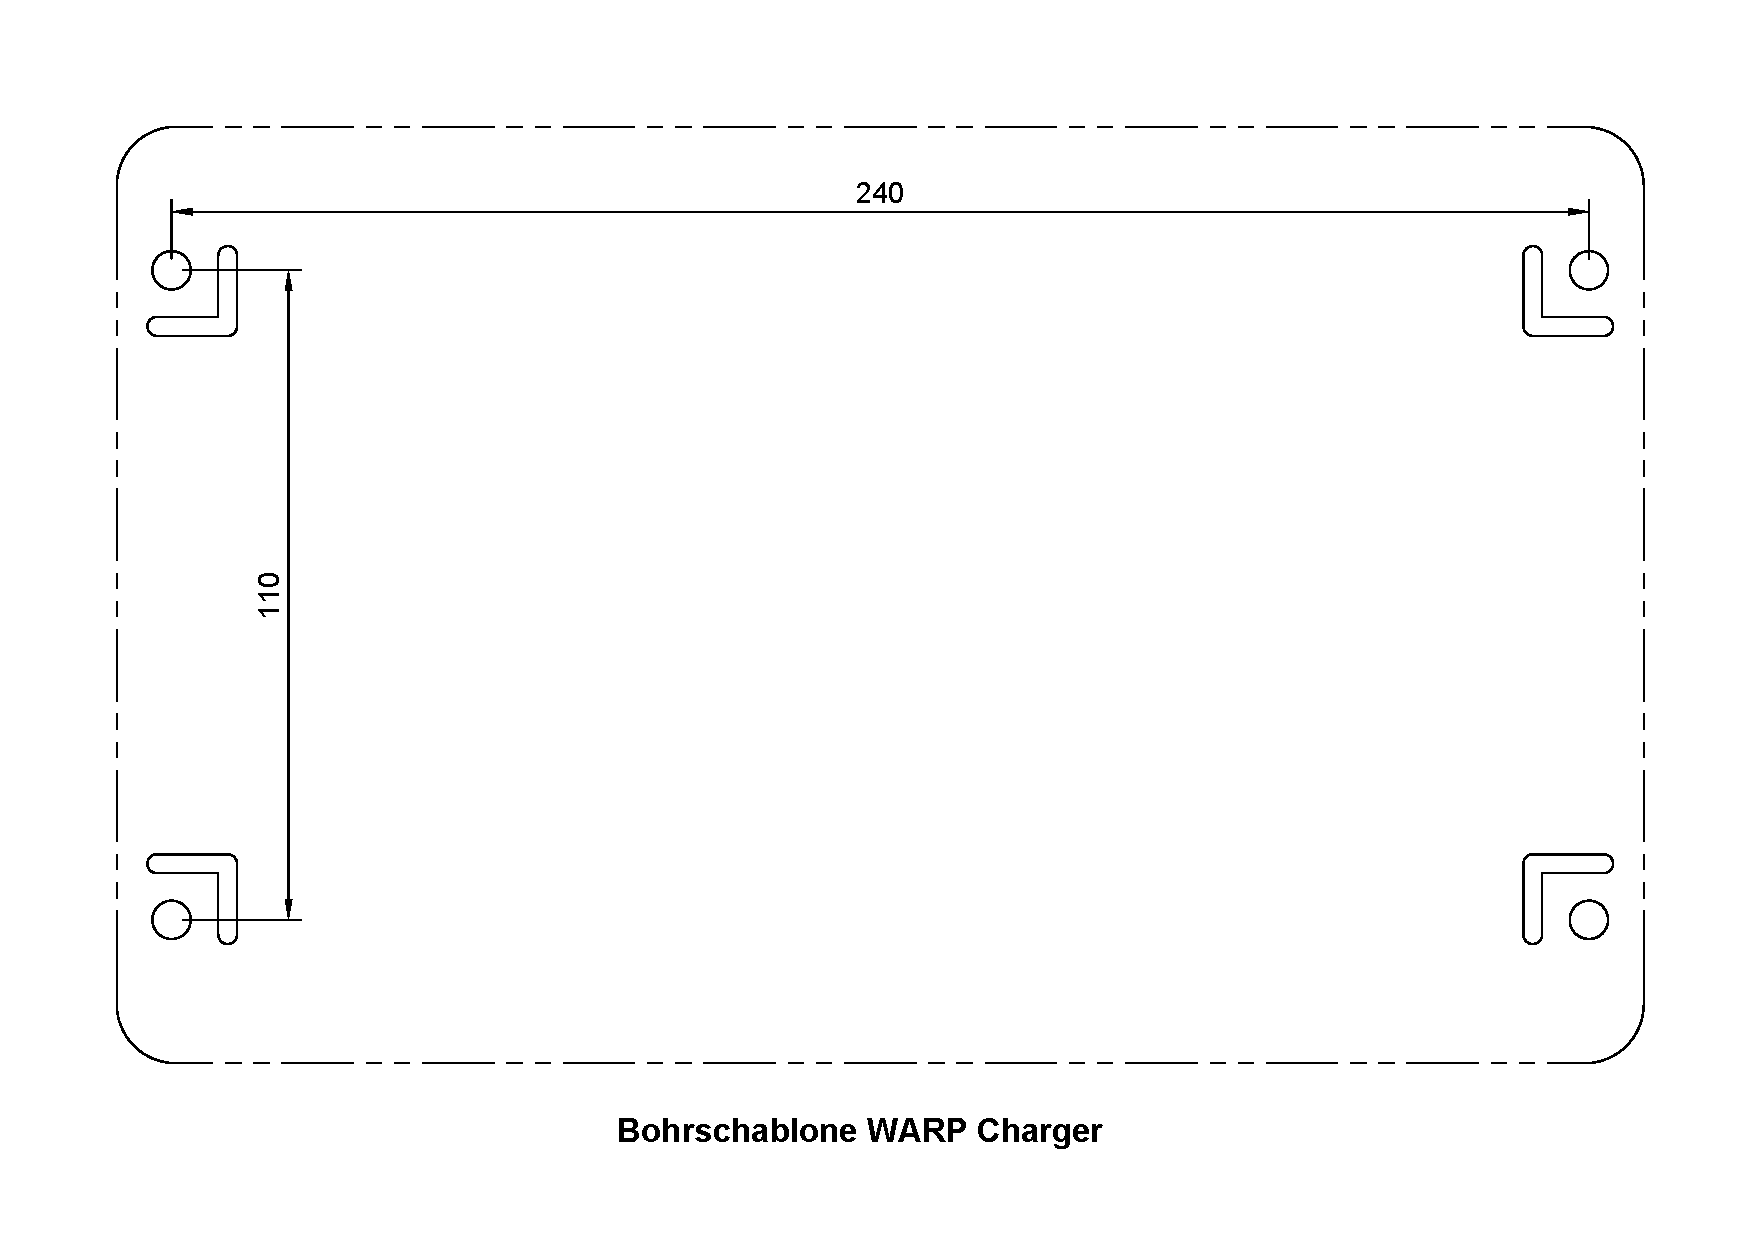
\includepdf{./img/resized/bohrschablone.pdf}
\end{document}
